%\documentclass[twocolumn,12pt]{IEEEtran}
%\documentclass[journal]{IEEEtran}
%\documentclass[conference,a4paper]{IEEEtran}
\documentclass[conference]{IEEEtran}
\IEEEoverridecommandlockouts
%\documentclass[draftclsnofoot,onecolumn,12pt]{IEEEtran}
\usepackage{cite}
\usepackage{algorithm,amsbsy,amsmath,amssymb,epsfig,bbm,mathrsfs,multirow,amsthm,amsfonts}
%\usepackage[a4paper]{}
%\usepackage[paperwidth=210mm,paperheight=297mm]{}
%\usepackage{array,multirow,graphicx}
\usepackage{array}
\usepackage{graphicx}
\usepackage{graphics}
\usepackage{subfigure}
\usepackage{epstopdf}
\usepackage{color}
\usepackage{soul}
\usepackage{bbm}
% adding
%\usepackage[utf8]{vietnam}
%\usepackage{comment}https://www.overleaf.com/project/62fde8f76bfde06d4d48297c
\usepackage{algpseudocode}
\usepackage{mathtools}
\usepackage{pdfpages}
\renewcommand{\algorithmicrequire}{\textbf{Input:}}
\renewcommand{\algorithmicensure}{\textbf{Output:}} 
\DeclareMathOperator{\Tr}{Tr}
%\usepackage{amsmath}

\clearpage{\pagestyle{empty}\cleardoublepage}
\pagestyle{empty}

% \oddsidemargin -0.3in
% \textwidth 7.025in
%\topmargin -0.45in
% \bottommargin 0.75in
%\textheight 9.3in
\renewcommand{\baselinestretch}{1.0}
\newcommand{\alglabel}[1]{\newcounter{#1}\setcounter{#1}{\value{ALC@line}}}
%\newcommand{\algref}[1]{\arabic{#1}}
\newcommand{\beq}{\begin{equation}}
\newcommand{\eeq}{\end{equation}}
\newcommand{\bitm}{\begin{itemize}}
\newcommand{\ba}{\begin{array}}
\newcommand{\ea}{\end{array}}
\newcommand{\eitm}{\end{itemize}}
\newcommand{\beqn}{\begin{eqnarray}}
\newcommand{\eeqn}{\end{eqnarray}}
\newcommand{\beqno}{\begin{eqnarray*}}
\newcommand{\eeqno}{\end{eqnarray*}}
\newcommand{\bma}{\begin{displaymath}}
\newcommand{\ema}{\end{displaymath}}
\newcommand{\bnu}{\begin{enumerate}}
\newcommand{\enu}{\end{enumerate}}
\newcommand{\bce}{\begin{center}}
\newcommand{\ece}{\end{center}}
\newcommand{\btb}{\begin{tabular}}
\newcommand{\etb}{\end{tabular}}
\newcommand{\tabincell}[2]{\begin{tabular}{@{}#1@{}}#2\end{tabular}}

\newtheorem{Definition}{\hskip 0pt Definition}%[section]
\newtheorem{lemma}{Lemma}
\newtheorem{observation}{Observation}
\newtheorem{theorem}{\textbf{\textsc{Theorem}}}
\newtheorem{mypro}{Proposition}
\hyphenation{lists}

% \begin{comment}
% \setlength\floatsep{0.7\baselineskip plus 3pt minus 2pt}
% \setlength\textfloatsep{0.7\baselineskip plus 3pt minus 2pt}
% \setlength\intextsep{0.7\baselineskip plus 3pt minus 2pt}
% \end{comment}

\usepackage{graphicx}
\usepackage{textcomp}
\usepackage{xcolor}
\def\BibTeX{{\rm B\kern-.05em{\sc i\kern-.025em b}\kern-.08em
    T\kern-.1667em\lower.7ex\hbox{E}\kern-.125emX}}

\begin{document}
\title{\huge Joint UAV trajectory, NOMA power allocation and BS deployment for energy-efficient SWIPT-enabled communications
}

\author{Hoang Cao Minh, Ninh Thi Thanh Tam,  Nguyen Minh Quan, and Trinh Van Chien
        % <-this % stops a space
%\thanks{(\textit{Corresponding author: Trinh Van Chien})}
\thanks{Ninh Thi-Thanh Tam is with Faculty of Information and Communication Technology, National Academy of Education Management, Vietnam and the School of Information and Communications Technology, Hanoi University of Science and Technology, Hanoi 100000, Vietnam (email: tam.ntt250098D@sis.hust.edu.vn)}

\thanks{ Hoang Cao Minh, Nguyen Minh Quan and Trinh Van Chien are with the School of Information and Communications Technology, Hanoi University of Science and Technology, Hanoi 100000, Vietnam (e-mail: minh.hc2416559@sis.hust.edu.vn, quannm@soict.hust.edu.vn,  chientv@soict.hust.edu.vn)}
}

\maketitle
\begin{abstract} The abstract of paper.
\end{abstract}
\begin{IEEEkeywords} UAV, PSO, SWIPT.
\end{IEEEkeywords}

\thispagestyle{empty}
\section{INTRODUCTION}
\label{sec:introduction}
The introduction part\\
In this paper, our main contributions are as follows:
\begin{itemize}
    \item We propose a joint optimization algorithm for UAV trajectory design to enhance wireless energy harvesting performance and compare its effectiveness with existing methods.
    \item We simultaneously optimize the base station deployment to improve the achievable sum rate of weak users in the considered system model.
    \item We refine the conventional Particle Swarm Optimization (PSO) algorithm to achieve better optimization performance and convergence efficiency.
\end{itemize}

%=============================

%=======================================
\section{SYSTEM MODEL AND 3D CHANNEL ASSUMPTIONS}
As illustrated in Fig. \ref{fig:1SystemModel}, we consider a UAV-assisted wireless communication network composed of base stations (BSs) and user equipment (UEs), employing both uplink and downlink non-orthogonal multiple access (NOMA) schemes. The UAV is equipped with simultaneous wireless information and power transfer (SWIPT) capabilities to enable energy harvesting during operation. The UAV moves from a predefined initial location to a designated final destination along an optimized trajectory. The objective is to maximize the minimum achievable downlink communication rate among all UEs while determining the optimal UAV trajectory.

\subsection{System Model}

\begin{figure*}[!t]
    \centering
\hspace{2mm} 
    %\subfloat[]
    {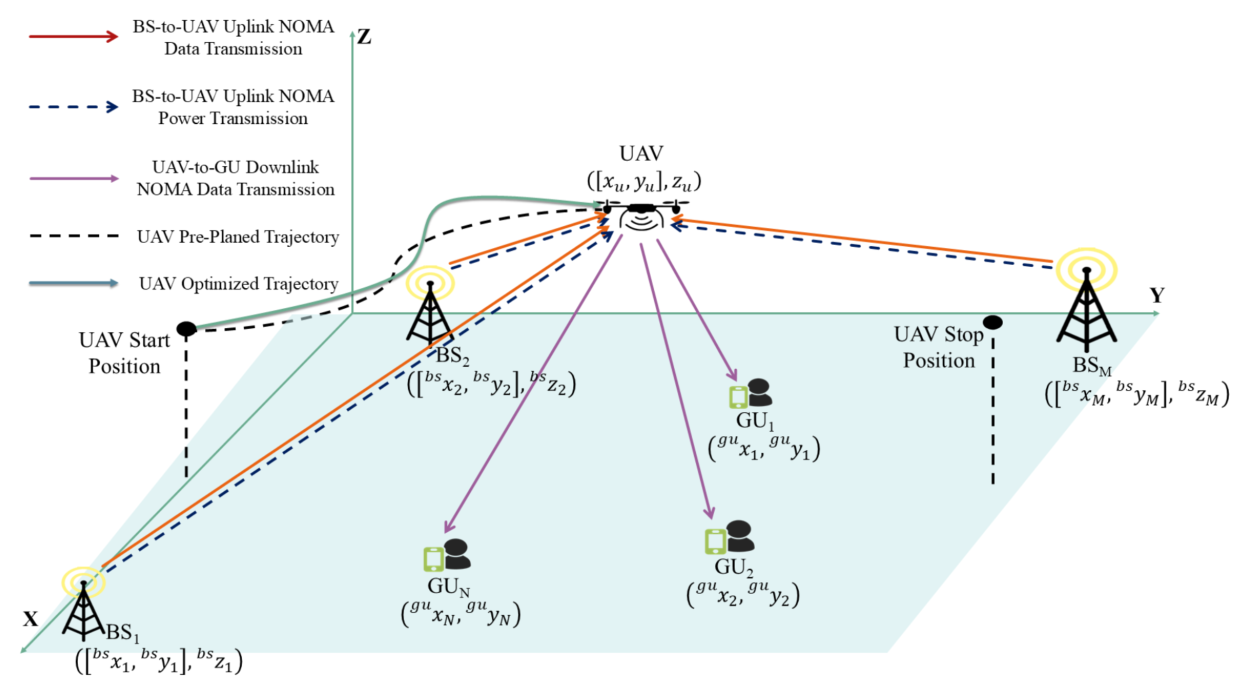
\includegraphics[width=0.8\textwidth]{Images/1SystemModel.png}}
    \label{fig:1SystemModel}
    \caption{System Model.}
\end{figure*}

As illustrated in the proposed system model shown in Fig. \ref{fig:1SystemModel}, a single UAV serves $N$ user equipment (UEs) while simultaneously establishing downlink NOMA links with the UEs and uplink NOMA links with $M$ base stations (BSs). The set of UEs is denoted by $\mathcal{N} = \{ 1, 2, \dots, N \}$, where the location of the $n$-th UE is represented as $\mathbf{UE}_n = [x_{n}^{UE}, y_{n}^{UE}, z_{n}^{UE}] \in \mathbb{R}^3, \forall n \in \mathcal{N}$, with $x_{n}^{UE}$ and $y_{n}^{UE}$ denoting the horizontal coordinates of the $n$-th UE in a three-dimensional (3D) Cartesian. We assume the user is on the ground, so $z_{n}^{UE} = 0$. 
Similarly, the set of BSs is denoted by $\mathcal{M} = \{ 1, 2, \dots, M\}$, where the position of the $m$-th BS is given by $\mathbf{BS}_m = [x_{m}^{BS}, y_{m}^{BS}, z_{m}^{BS}]$. Each BS is mounted on a supporting structure at a fixed altitude $z_{m}^{BS} > 0$, which is dictated by the deployment site and is therefore not subject to optimization. In contrast, the horizontal coordinates $x_{m}^{BS}$ and $y_{m}^{BS}$ are treated as design variables, since relocating a BS within its allowed deployment region alters the uplink channel towards the UAV and hence the amount of energy that can be harvested.

During operation, the UAV follows a predefined trajectory between specified initial and final locations. The UAV position is represented by $[x^{UAV}, y^{UAV}, z^{UAV}]$, which denotes the coordinates of the UAV.

As depicted in Fig.\ref{fig:1SystemModel}, the uplink communication corresponds to data transmission from the BSs to the UAV, whereas the downlink communication corresponds to data transmission from the UAV to the UEs. Moreover, the UAV employs simultaneous wireless information and power transfer (SWIPT) during uplink reception to harvest energy from the received BS signals, thereby supporting its energy consumption for downlink communications.

\subsection{Channel Assumptions}
\label{subsec:channel_assumptions}

The communication network under consideration consists of two wireless
links: the uplink from the $m$-th BS to the UAV and the downlink from the
UAV to the $n$-th UE. The corresponding channel coefficients are denoted
by $h_n$ and $k_m$, respectively. Both are air-to-ground links in which
the line-of-sight (LoS) component is typically dominant but is not
guaranteed. Accordingly, we adopt a Rician fading model whose $K$-factor
depends on the elevation angle between the UAV and the corresponding
ground node.

At mission step $t$, let the UAV be located at
$\mathbf{q}_t=[x_t^{\mathrm{UAV}},y_t^{\mathrm{UAV}},z_t^{\mathrm{UAV}}]^T$,
which is abbreviated as $(x_t,y_t,z_t)$ throughout this subsection for
notational brevity. Since the UEs are located on the ground, i.e.,
$z_n^{\mathrm{UE}}=0$, the horizontal distance, the three-dimensional
distance and the elevation angle from UE $n$ to the UAV are respectively
given by
\begin{equation}
\begin{aligned}
d_{t,n}^{\mathrm{UE}}&=\sqrt{\big(x_t-x_n^{\mathrm{UE}}\big)^{2}
      +\big(y_t-y_n^{\mathrm{UE}}\big)^{2}},\\
r_{t,n}^{\mathrm{UE}}&=\sqrt{\big(d_{t,n}^{\mathrm{UE}}\big)^{2}+z_t^{2}},\\
\theta_{t,n}^{\mathrm{UE}}&=\arctan\!\big(z_t\big/d_{t,n}^{\mathrm{UE}}\big)
      \in\big[0,\tfrac{\pi}{2}\big].
\end{aligned}
\end{equation}
The corresponding quantities for the uplink from BS $m$ follow by
analogy, the only difference being that each BS has a fixed nonzero
altitude $z_m^{\mathrm{BS}}$:
\begin{equation}
\begin{aligned}
d_{t,m}^{\mathrm{BS}}&=\sqrt{\big(x_t-x_m^{\mathrm{BS}}\big)^{2}
      +\big(y_t-y_m^{\mathrm{BS}}\big)^{2}},\\
r_{t,m}^{\mathrm{BS}}&=\sqrt{\big(d_{t,m}^{\mathrm{BS}}\big)^{2}
      +\big(z_m^{\mathrm{BS}}-z_t\big)^{2}},\\
\theta_{t,m}^{\mathrm{BS}}&=\arctan\!\big(\big|z_m^{\mathrm{BS}}-z_t\big|
      \big/d_{t,m}^{\mathrm{BS}}\big).
\end{aligned}
\end{equation}
It is worth noting that $d_{t,m}^{\mathrm{BS}}$ depends on the horizontal
BS coordinates $x_m^{\mathrm{BS}}$ and $y_m^{\mathrm{BS}}$, which are
treated as optimization variables in this work. Consequently, the uplink
channel quality, and therefore the amount of energy harvested by the UAV,
can be actively improved through BS deployment.

The large-scale channel power gains of the two links follow the standard
distance-dependent model
\begin{equation}
\beta_{t,n}^{\mathrm{UE}}
=\beta_{0}\big(r_{t,n}^{\mathrm{UE}}\big)^{-\eta},
\qquad
\beta_{t,m}^{\mathrm{BS}}
=\beta_{0}\big(r_{t,m}^{\mathrm{BS}}\big)^{-\eta},
\end{equation}
where $\beta_{0}$ denotes the reference channel power gain at a distance
of one meter and $\eta$ is the path loss exponent.

The small-scale fading coefficient of each link is modeled as a Rician
random variable consisting of a deterministic LoS component and a random
non-line-of-sight (NLoS) component. Writing
$K_{t,n}^{\mathrm{UE}}=K\big(\theta_{t,n}^{\mathrm{UE}}\big)$, the
downlink coefficient to UE $n$ is
\begin{equation}
g_{t,n}
=\sqrt{\frac{K_{t,n}^{\mathrm{UE}}}{K_{t,n}^{\mathrm{UE}}+1}}\;\bar{g}
+\sqrt{\frac{1}{K_{t,n}^{\mathrm{UE}}+1}}\;\tilde{g}_{n},
\end{equation}
where $\bar{g}$ is the deterministic LoS component with $|\bar{g}|=1$ and
$\tilde{g}_{n}\sim\mathcal{CN}(0,1)$ is the NLoS component. The uplink
coefficient $g_{t,m}$ is obtained in the same manner by replacing
$K_{t,n}^{\mathrm{UE}}$ with $K_{t,m}^{\mathrm{BS}}$ and $\tilde{g}_{n}$
with $\tilde{g}_{m}$.

The Rician $K$-factor is an increasing function of the elevation angle,
since a larger elevation angle reduces the probability of blockage by
ground obstacles. Following the widely adopted exponential model,
% TODO: them \cite{...} cho mo hinh he so K theo ham mu o cau tren.
we set
\begin{equation}
K(\theta)=A_{1}\exp\!\big(A_{2}\,\theta\big),
\qquad \theta\in\big[0,\tfrac{\pi}{2}\big],
\end{equation}
where the two environment-specific constants are determined by the
$K$-factor values at the two extreme elevation angles, namely
$A_{1}=K_{\min}$ and
$A_{2}=\frac{2}{\pi}\ln\!\big(K_{\max}/K_{\min}\big)$, so that
$K(0)=K_{\min}$ when the UAV is seen at the horizon and
$K(\pi/2)=K_{\max}$ when it is directly overhead.

Combining the large-scale and small-scale components, the downlink
channel coefficient from the UAV to UE $n$ and the uplink channel
coefficient from BS $m$ to the UAV at mission step $t$ are respectively
expressed as
\begin{equation}
h_{t,n}=\sqrt{\beta_{t,n}^{\mathrm{UE}}}\;g_{t,n},
\qquad
k_{t,m}=\sqrt{\beta_{t,m}^{\mathrm{BS}}}\;g_{t,m}.
\end{equation}

Two remarks are in order. First, the small-scale fading coefficients
$\tilde{g}_{n}$ and $\tilde{g}_{m}$ are assumed to remain constant over
the whole UAV mission, i.e., a quasi-static block fading model is
adopted. This assumption isolates the effect of the UAV trajectory and
the BS deployment on the achievable performance from the effect of
random fading fluctuations, so that the performance gaps reported in
Section~V can be attributed to the optimization algorithms rather than to
favourable fading realizations. Independent fading realizations are
instead generated across the Monte Carlo runs.

Second, the channel power gain
$|h_{t,n}|^{2}=\beta_{0}\big(r_{t,n}^{\mathrm{UE}}\big)^{-\eta}
|g_{t,n}|^{2}$ exhibits two competing dependencies on the UAV altitude.
Increasing $z_t$ enlarges the elevation angle and hence the Rician
$K$-factor, which improves the reliability of the link; however, it
simultaneously increases the three-dimensional distance
$r_{t,n}^{\mathrm{UE}}$ and therefore aggravates the path loss. The
resulting trade-off is non-monotonic in the UAV position and constitutes
one of the sources of non-convexity of the optimization problem
formulated in Section~III-B.



%=======================================
\section{PERFORMANCE METRICS AND OPTIMIZATION PROBLEM}

\subsection{Performance Metrics}
\label{subsec:performance_metrics}

This subsection specifies the quantities used to evaluate the system,
following the signal flow from the energy harvested at the UAV to the
rates delivered to the UEs. All quantities are defined independently of
the optimization algorithm, so that the same metrics apply to every
scheme compared in Section~\ref{sec:results}.

At mission step $t$, the UAV simultaneously receives the signals
transmitted by all $M$ BSs, each with transmit power $P^{\mathrm{BS}}$.
Applying the linear energy harvesting model over a slot of duration
$T_{s}$, the energy collected by the UAV is
\begin{equation}
\label{eq:harvested_energy}
E_{t}=\varphi\,\zeta\,P^{\mathrm{BS}}
      \sum_{m=1}^{M}\big|k_{t,m}\big|^{2}\,T_{s},
\end{equation}
where $\varphi\in(0,1]$ is the fraction of the received power routed to
the energy harvesting circuit and $\zeta\in(0,1]$ is the RF-to-DC
conversion efficiency. The harvested energy is entirely consumed for
downlink transmission within the same slot, so the transmit power
available to the UAV is
\begin{equation}
\label{eq:uav_power}
P_{t}=\frac{E_{t}}{T_{s}}
     =\varphi\,\zeta\,P^{\mathrm{BS}}
      \sum_{m=1}^{M}\big|k_{t,m}\big|^{2}.
\end{equation}
Equation~\eqref{eq:uav_power} is central to the proposed design: the
downlink transmit power is \emph{linearly} proportional to the aggregate
uplink channel power gain. Since $|k_{t,m}|^{2}$ depends on the BS
coordinates through $d_{t,m}^{\mathrm{BS}}$, relocating the BSs directly
scales the power budget of every downlink transmission. This is what
makes the BS positions worth optimizing jointly with the trajectory,
rather than treating them as fixed infrastructure.

The UAV serves the $N$ UEs by superposition coding, and each UE applies
successive interference cancellation (SIC). Let $\pi_{t}(\cdot)$ denote
the permutation that sorts the UEs by ascending channel power gain at
step $t$, i.e.,
\begin{equation}
\label{eq:sic_order}
\big|h_{t,\pi_{t}(1)}\big|^{2}\le
\big|h_{t,\pi_{t}(2)}\big|^{2}\le\cdots\le
\big|h_{t,\pi_{t}(N)}\big|^{2}.
\end{equation}
For brevity we write $[u]$ in place of $\pi_{t}(u)$. Following the NOMA
decoding principle, the UE with the weakest channel is decoded first and
treats the signals of all stronger UEs as interference, whereas the UE
with the strongest channel is decoded last and, under the assumption of
perfect SIC, experiences no intra-cluster interference. The resulting
signal-to-interference-plus-noise ratio of the $u$-th UE in the decoding
order is
\begin{equation}
\label{eq:sinr}
\gamma_{t,[u]}
=\frac{P_{t}\,\alpha_{t,[u]}\big|h_{t,[u]}\big|^{2}}
      {N_{0}+P_{t}\big|h_{t,[u]}\big|^{2}
       \sum_{j=u+1}^{N}\alpha_{t,[j]}},
\end{equation}
where $\alpha_{t,n}$ is the power allocation coefficient assigned to UE
$n$ at step $t$, $N_{0}$ is the noise power over the signal bandwidth
$B$, and the summation is taken to be zero for $u=N$. The corresponding
achievable rate of UE $n$ at step $t$ is
\begin{equation}
\label{eq:rate}
R_{t,n}=B\log_{2}\big(1+\gamma_{t,n}\big).
\end{equation}

Since the UAV has fixed initial and final positions, the system is
assessed only over the internal mission steps
\begin{equation}
\label{eq:internal_steps}
\mathcal{T}_{\mathrm{int}}=\{2,3,\ldots,T-1\},
\end{equation}
so that $|\mathcal{T}_{\mathrm{int}}|=T-2$. At each such step, the
performance of the worst-served UE is
\begin{equation}
\label{eq:step_min_rate}
R_{t}^{\min}=\min_{n\in\mathcal{N}}R_{t,n},
\end{equation}
and the two aggregate rate metrics of interest are the worst and the
average value of $R_{t}^{\min}$ along the mission,
\begin{equation}
\label{eq:rate_aggregates}
R_{\min}=\min_{t\in\mathcal{T}_{\mathrm{int}}}R_{t}^{\min},
\qquad
\bar{R}_{\min}=\frac{1}{|\mathcal{T}_{\mathrm{int}}|}
\sum_{t\in\mathcal{T}_{\mathrm{int}}}R_{t}^{\min}.
\end{equation}
The quantity $R_{\min}$ is the primary design target, as it characterizes
the service level guaranteed throughout the whole mission, while
$\bar{R}_{\min}$ describes the typical rather than the worst behaviour
and therefore distinguishes solutions that share the same bottleneck
step.

Because $R_{\min}$ and $\bar{R}_{\min}$ are both determined by the
worst-served UE alone, they are insensitive to how the remaining UEs are
treated. To capture this, the Jain fairness index is evaluated at each
internal step,
\begin{equation}
\label{eq:jain}
J_{t}=\frac{\big(\sum_{n=1}^{N}R_{t,n}\big)^{2}}
           {N\sum_{n=1}^{N}R_{t,n}^{2}+\epsilon},
\qquad t\in\mathcal{T}_{\mathrm{int}},
\end{equation}
where $\epsilon$ is a small positive constant that prevents division by
zero. The index satisfies $J_{t}\in(0,1]$, attaining $J_{t}=1$ when all
UEs receive identical rates; a lower value indicates a more unbalanced
allocation.

Finally, because the transmit power is harvested rather than supplied
from an onboard source, the average power actually available to the UAV,
\begin{equation}
\label{eq:avg_power}
\bar{P}=\frac{1}{|\mathcal{T}_{\mathrm{int}}|}
\sum_{t\in\mathcal{T}_{\mathrm{int}}}P_{t},
\end{equation}
is reported as a separate metric. It measures how effectively a given
trajectory and BS deployment exploit the energy available in the uplink,
and it isolates the contribution of the energy harvesting mechanism from
that of the power allocation.

\subsection{Problem Formulation}
\label{subsec:problem_formulation}

The design variables of the joint optimization problem are the internal
UAV trajectory coordinates, the downlink NOMA power allocation matrix and
the horizontal BS coordinates, collected as
\begin{equation}
\label{eq:variable_set}
\mathcal{X}=\big\{\mathbf{x}^{\mathrm{UAV}},\,\mathbf{z}^{\mathrm{UAV}},\,
\mathbf{A}_{\alpha},\,\mathbf{x}^{\mathrm{BS}},\,
\mathbf{y}^{\mathrm{BS}}\big\}.
\end{equation}
Guided by the metrics of Section~\ref{subsec:performance_metrics}, the
design goal is to maximize the rate delivered to the worst-served UE at
the worst mission step, so that a service level is guaranteed uniformly
in both dimensions. Writing $(x_{t},z_{t})$ for the UAV coordinates at
step $t$ as in Section~\ref{subsec:channel_assumptions}, the problem is
stated as
\begin{subequations}
\label{eq:P1}
\begin{align}
(\mathrm{P1}):\quad
\max_{\mathcal{X}}\;\;
& \min_{t\in\mathcal{T}_{\mathrm{int}}}\;\min_{n\in\mathcal{N}} R_{t,n}
  \label{eq:P1_obj}\\
\mathrm{s.t.}\;\;
& x_{\min}^{\mathrm{UAV}}\le x_{t}\le x_{\max}^{\mathrm{UAV}},
  \;\forall t\in\mathcal{T}_{\mathrm{int}}, \label{eq:c_xbound}\\
& z_{\min}^{\mathrm{UAV}}\le z_{t}\le z_{\max}^{\mathrm{UAV}},
  \;\forall t\in\mathcal{T}_{\mathrm{int}}, \label{eq:c_zbound}\\
& |x_{t}-x_{t-1}|\le\Delta x_{\max},\;\forall t\ge2,
  \label{eq:c_movex}\\
& |z_{t}-z_{t-1}|\le\Delta z_{\max},\;\forall t\ge2,
  \label{eq:c_movez}\\
& \mathbf{q}_{1}=\mathbf{q}_{\mathrm{S}},\quad
  \mathbf{q}_{T}=\mathbf{q}_{\mathrm{E}}, \label{eq:c_endpoints}\\
& \sum_{n=1}^{N}\alpha_{t,n}=1,\;\alpha_{t,n}\ge\alpha_{\min},
  \label{eq:c_alpha}\\
& |h_{t,i}|^{2}\le|h_{t,j}|^{2}\Rightarrow\alpha_{t,i}\ge\alpha_{t,j},
  \label{eq:c_noma}\\
& x_{m,\min}^{\mathrm{BS}}\le x_{m}^{\mathrm{BS}}
  \le x_{m,\max}^{\mathrm{BS}},\;\forall m\in\mathcal{M},
  \label{eq:c_bsx}\\
& y_{m,\min}^{\mathrm{BS}}\le y_{m}^{\mathrm{BS}}
  \le y_{m,\max}^{\mathrm{BS}},\;\forall m\in\mathcal{M},
  \label{eq:c_bsy}\\
& P_{t}=\varphi\,\zeta\,P^{\mathrm{BS}}
  \sum_{m=1}^{M}|k_{t,m}|^{2}. \label{eq:c_power}
\end{align}
\end{subequations}
Unless stated otherwise, \eqref{eq:c_alpha} holds for every UE $n$ and
every step $t$, \eqref{eq:c_noma} for every pair of UEs $i,j$ at every
step $t$, and \eqref{eq:c_power} for every
$t\in\mathcal{T}_{\mathrm{int}}$.

Constraints \eqref{eq:c_xbound} and \eqref{eq:c_zbound} confine the UAV
to the admissible flying region, while \eqref{eq:c_movex} and
\eqref{eq:c_movez} limit the displacement between consecutive mission
steps and thus encode the finite manoeuvring capability of the platform.
Constraint \eqref{eq:c_endpoints} fixes the take-off and landing points
$\mathbf{q}_{\mathrm{S}}$ and $\mathbf{q}_{\mathrm{E}}$ imposed by the
mission. Constraint \eqref{eq:c_alpha} normalizes the power allocation
and reserves a minimum share $\alpha_{\min}>0$ for every UE, which
prevents a UE from being switched off entirely in order to inflate the
rates of the others. Constraint \eqref{eq:c_noma} enforces the NOMA
principle that a UE with a weaker channel must receive a larger power
share, and \eqref{eq:c_bsx}--\eqref{eq:c_bsy} restrict each BS to its
admissible deployment region. Finally, \eqref{eq:c_power} is not a
design restriction but a coupling relation: it states that the transmit
power entering \eqref{eq:sinr} is not a free variable but is produced by
the uplink channels, and therefore by the BS coordinates.

Problem $(\mathrm{P1})$ is difficult to solve by classical convex
optimization for four distinct reasons.

First, the objective is non-convex in the UAV coordinates. The channel
power gain combines a distance-dependent path loss with a Rician
$K$-factor that varies exponentially with the elevation angle, and
Section~\ref{subsec:channel_assumptions} showed that the two act in
opposite directions as the altitude changes.

Second, the variable groups are mutually coupled. Through
\eqref{eq:c_power} the BS coordinates determine the power budget of
every downlink transmission, and the UAV trajectory simultaneously
shapes the uplink and the downlink channels. The problem therefore does
not decompose into independent subproblems that could be solved
separately and recombined.

Third, and most restrictive, the SIC decoding order is a combinatorial
function of the trajectory. The permutation $\pi_{t}$ defined in
\eqref{eq:sic_order} changes whenever the UAV crosses a locus along
which two UEs have equal channel gains, and at such a crossing the power
shares dictated by \eqref{eq:c_noma} are exchanged between those two
UEs. Consequently $R_{t,n}$ is not merely non-convex in the trajectory
variables but \emph{discontinuous} in them, and \eqref{eq:c_noma} acts as
a combinatorial rather than a continuous constraint. Gradient-based
methods and successive convex approximation, which both presuppose at
least local smoothness, are not applicable without fixing the decoding
order in advance, which would in turn exclude part of the search space.

Fourth, the doubly nested $\min$ operator in \eqref{eq:P1_obj} is
non-smooth, so that the objective exhibits kinks wherever the identity of
the bottleneck UE or of the bottleneck mission step changes.

For these reasons we do not attempt an exact solution of
$(\mathrm{P1})$ and instead adopt the population-based search described
in Section~\ref{sec:algorithms}, which requires only function
evaluations and therefore tolerates both the discontinuity and the
non-smoothness.

One further observation motivates the formulation actually used by the
algorithm. Because \eqref{eq:P1_obj} depends solely on the worst-served
UE, it is indifferent to the treatment of the remaining UEs: two designs
attaining the same $R_{\min}$ are deemed equivalent even if one
distributes the rates evenly while the other leaves several UEs close to
the bottleneck. To resolve this ambiguity in favour of balanced designs,
the search in Section~\ref{sec:algorithms} operates on a scalarized
surrogate of $(\mathrm{P1})$ that augments \eqref{eq:P1_obj} with the
average minimum rate $\bar{R}_{\min}$ and with a penalty built on the
Jain index \eqref{eq:jain}, while the constraints
\eqref{eq:c_xbound}--\eqref{eq:c_bsy} are enforced by a repair operator
combined with a violation penalty.


%=============================
\section{PROPOSED ALGORITHMS}
\label{sec:algorithms}

\subsection{Overview of the Proposed Joint Optimization Framework}
\label{subsec:algorithm_overview}
In the considered SWIPT-enabled UAV-assisted NOMA system, the communication performance depends on several strongly coupled factors, including the UAV trajectory, the downlink NOMA power allocation coefficients, and the BSs' positions. The UAV trajectory affects both the UAV-to-UE downlink channels and the BS-to-UAV uplink channels. Meanwhile, the harvested energy from the BS signals determines the available transmit power at the UAV for downlink transmission. Therefore, optimizing only the UAV trajectory may not fully exploit the potential of the system, especially when the BS deployment and power allocation strategy also influence the achievable rates of the UEs.

To address this issue, we formulate a joint optimization framework that simultaneously considers UAV trajectory design, NOMA power allocation, and BS position adjustment. The main objective is to improve the worst-user performance along the UAV mission by maximizing the minimum achievable downlink rate among all UEs. In addition, user fairness is also considered to avoid a situation where only one or two users obtain high rates while the remaining users experience poor service quality. This objective is suitable for NOMA-based systems because users may experience significantly different channel conditions depending on their distances and channel gains with respect to the UAV. Therefore, the proposed framework aims not only to enhance the minimum achievable rate, but also to maintain a more balanced rate distribution among the UEs.

The resulting optimization problem is challenging due to the non-convex relationship between the UAV position, channel gain, harvested energy, interference in NOMA transmission, and achievable rate. Moreover, the optimization variables include continuous trajectory coordinates, power allocation coefficients across mission steps, and BS horizontal positions. Therefore, instead of relying on conventional convex optimization methods, we employ a PSO-based metaheuristic approach to search for high-quality feasible solutions. In the proposed framework, each particle represents a complete candidate design of the UAV trajectory, the power allocation coefficients, and the BS positions. The quality of each particle is evaluated using a fitness function based on the minimum achievable rate and additional penalty terms for constraint violations.
\subsection{Solution Representation}
\label{subsec:solution_representation}

In the proposed joint optimization framework, each candidate solution represents a complete configuration of the UAV trajectory, the downlink NOMA power allocation variables, and the horizontal positions of the BSs. Let $T$ denote the number of mission steps, $N$ denote the number of UEs, and $M$ denote the number of BSs. Since the UAV has predefined initial and final positions, only the internal trajectory points are included in the optimization process. At mission step $t$, the UAV position is denoted by 
\begin{equation} 
\mathbf{q}_t = 
\left[ 
x_t^{\mathrm{UAV}}, 
y_t^{\mathrm{UAV}}, 
z_t^{\mathrm{UAV}} 
\right]^T 
\in \mathbb{R}^{3}, 
\quad t = 1,2, \ldots,T. 
\end{equation} 
The initial and final UAV positions, $\mathbf{q}_1$ and $\mathbf{q}_T$, are fixed. In this work, the UAV moves along the mission direction with predefined $y$-coordinates. Therefore, only the internal $x$- and $z$-coordinates of the UAV are optimized. These variables are represented as \begin{equation} \mathbf{x}^{\mathrm{UAV}} = \left[ x_2^{\mathrm{UAV}}, x_3^{\mathrm{UAV}}, \ldots, x_{T-1}^{\mathrm{UAV}} \right]^T \in \mathbb{R}^{T-2}, 
\end{equation} 
and 
\begin{equation} \mathbf{z}^{\mathrm{UAV}} = \left[ z_2^{\mathrm{UAV}}, z_3^{\mathrm{UAV}}, \ldots, z_{T-1}^{\mathrm{UAV}} \right]^T \in \mathbb{R}^{T-2}. 
\end{equation} 
After decoding the solution vector, the complete UAV trajectory is reconstructed by combining the fixed endpoints with the optimized internal coordinates. For the downlink NOMA transmission, the power allocation vector at mission step $t$ is denoted by 
\begin{equation} \boldsymbol{\alpha}_t = \left[ \alpha_{t,1}, \alpha_{t,2}, \ldots, \alpha_{t,N} \right]^T \in \mathbb{R}^{N}, \end{equation} 
where $\alpha_{t,n}$ is the power allocation coefficient assigned to UE $n$ at step $t$. The power allocation variables over all mission steps are arranged into the following matrix: 
\begin{equation} \mathbf{A}_{\alpha} = \left[ \begin{array}{c} \boldsymbol{\alpha}_1^T \\ \boldsymbol{\alpha}_2^T \\ \vdots \\ \boldsymbol{\alpha}_T^T \end{array} \right] \in \mathbb{R}^{T \times N}. \end{equation} 

For particle-based optimization, this matrix is further vectorized in a row-wise manner as
\begin{equation}
\mathbf{a} = \left[ \alpha_{1,1},\ldots,\alpha_{1,N}, \ldots, \alpha_{T,1},\ldots,\alpha_{T,N} \right]^T \in \mathbb{R}^{TN}.
\end{equation}

The entries in this block are repaired during the optimization process so that the resulting power allocation coefficients satisfy the NOMA power allocation requirements. In addition to the UAV trajectory and power allocation variables, the horizontal positions of the BSs are also optimized. The BS position variables are represented as 
\begin{equation} \mathbf{x}^{\mathrm{BS}} = \left[ x_1^{\mathrm{BS}}, x_2^{\mathrm{BS}}, \ldots, x_M^{\mathrm{BS}} \right]^T \in \mathbb{R}^{M}, \end{equation} 
and 
\begin{equation} \mathbf{y}^{\mathrm{BS}} = \left[ y_1^{\mathrm{BS}}, y_2^{\mathrm{BS}}, \ldots, y_M^{\mathrm{BS}} \right]^T \in \mathbb{R}^{M}. \end{equation} 
The altitude of each BS is fixed and is not included in the optimization variables. Therefore, each candidate solution, corresponding to the position of a particle in the PSO/IPSO search space, is encoded as the following real-valued decision vector $\mathbf{s} \in \mathbb{R}^{D}$: 
\begin{equation}
\mathbf{s} = \big[ (\mathbf{x}^{\mathrm{UAV}})^T, (\mathbf{z}^{\mathrm{UAV}})^T, \mathbf{a}^T, (\mathbf{x}^{\mathrm{BS}})^T, (\mathbf{y}^{\mathrm{BS}})^T \big]^T,
\end{equation} 
where the dimension of the solution vector is 
\begin{equation} D = 2(T-2) + TN + 2M. \end{equation} 
Here, $2(T-2)$ corresponds to the internal UAV trajectory variables, $TN$ corresponds to the power allocation variables over all mission steps and users, and $2M$ corresponds to the horizontal BS position variables. This stacked vector representation enables the proposed algorithm to jointly optimize the UAV trajectory, the NOMA power allocation, and the BS deployment in a unified search process.

\subsection{Fitness Function Design}
\label{subsec:fitness_function}

For each candidate solution, the UAV trajectory, the NOMA power allocation coefficients, and the BS positions are first decoded from the solution vector. Then, the BS-to-UAV and UAV-to-UE channel coefficients are calculated at each mission step according to the adopted channel model. Based on the received signals from the BSs, the harvested energy at the UAV is computed and converted into the UAV transmit power for downlink NOMA transmission.

The fitness function is assembled from the performance metrics introduced in Section~\ref{subsec:performance_metrics}. Besides maximizing the worst-case rate $R_{\min}$ of \eqref{eq:rate_aggregates}, the proposed design rewards the average minimum rate $\bar{R}_{\min}$ and discourages unbalanced rate allocation among the UEs by means of the Jain index $J_t$ of \eqref{eq:jain}. The fairness penalty is defined as

\begin{equation}
P_{\mathrm{fair}}
=
\lambda_{\mathrm{fair}}
\bar{R}_{\min}
\frac{1}{|\mathcal{T}_{\mathrm{int}}|}
\sum_{t \in \mathcal{T}_{\mathrm{int}}}
(1-J_t),
\end{equation}
where $\lambda_{\mathrm{fair}}$ is the fairness weighting factor.

The final fitness function is defined as
\begin{equation}
F
=
R_{\min}
+
\lambda_{\mathrm{mean}}
\bar{R}_{\min}
-
P_{\mathrm{fair}}
-
P_{\mathrm{c}},
\end{equation}
where $\lambda_{\mathrm{mean}}$ controls the contribution of the average minimum rate, and $P_{\mathrm{c}}$ is the constraint violation penalty. The penalty term $P_{\mathrm{c}}$ is applied when a candidate solution violates the UAV flying region, the UAV movement constraints, or the BS deployment bounds.

This fitness function encourages the algorithm to improve the worst-user performance over the whole trajectory, while also avoiding highly unbalanced rate allocation among the UEs. Therefore, the selected solution is expected to provide both a higher minimum achievable rate and better fairness among users.
\subsection{Constraint Handling and Solution Repair}
\label{subsec:constraint_handling}

Since the particle update process may generate infeasible candidate solutions, a repair mechanism is applied after each position update. The purpose of this mechanism is to ensure that all optimization variables remain within their feasible domains before evaluating the fitness value.

First, the UAV trajectory variables are repaired according to the allowed flying region. Whenever an internal coordinate violates the box constraints \eqref{eq:c_xbound} or \eqref{eq:c_zbound}, it is projected back to the nearest feasible value. The mobility constraints \eqref{eq:c_movex} and \eqref{eq:c_movez} are then enforced by forward and backward repair passes along the trajectory, which also preserve the fixed endpoints required by \eqref{eq:c_endpoints}.

Second, the NOMA power allocation coefficients are repaired at every mission step. The raw values are first clipped from below by $\alpha_{\min}$ and then normalized so that \eqref{eq:c_alpha} holds. To satisfy the NOMA ordering requirement \eqref{eq:c_noma}, the normalized coefficients are finally rearranged according to the channel-gain order of the UEs at that step, so that a UE with a weaker channel never receives a smaller power share than a stronger one.

Third, the BS horizontal positions are clipped to their admissible deployment regions \eqref{eq:c_bsx} and \eqref{eq:c_bsy}. The altitude of each BS is fixed and is not included in the repair process.

Although the repair mechanism is applied to improve feasibility, a constraint violation penalty is still included in the fitness function. This penalty discourages infeasible solutions and stabilizes the search process. In the proposed algorithm, no additional post-processing step is applied after the PSO/IPSO search; the final solution is directly obtained from the best repaired particle found during the optimization process.

\subsection{Joint PSO-Based Optimization}
\label{subsec:joint_pso}

After defining the solution representation, fitness function, and constraint-handling mechanism, the joint optimization problem is solved using a PSO-based search procedure. In this subsection, the term ``joint'' refers to the fact that each particle simultaneously contains the UAV trajectory variables, the downlink NOMA power allocation variables, and the BS horizontal position variables. The particle update itself follows the standard PSO mechanism, while the improved PSO variant will be introduced in the next subsection. Let $S$ denote the swarm size and $I_{\max}$ denote the maximum number of iterations. At iteration $i$, the position of the $k$-th particle is denoted by 
\begin{equation} 
\mathbf{s}_k^{(i)} \in \mathbb{R}^{D}, 
\quad k = 1,2,\ldots,S, 
\end{equation} 
where $D$ is the dimension of the joint solution vector defined in Section~\ref{subsec:solution_representation}. The velocity of the corresponding particle is denoted by $\mathbf{v}_k^{(i)} \in \mathbb{R}^{D}$. Each particle position is decoded into the UAV trajectory, the power allocation coefficients, and the BS positions before fitness evaluation. The initial swarm is generated within the predefined search ranges. To improve the stability of the search process, a feasible baseline solution can also be included as one initial particle. After initialization, each particle is processed by the repair operator $\mathcal{R}(\cdot)$ described in Section~\ref{subsec:constraint_handling}. The repaired particle is then evaluated using the fitness function defined in Section~\ref{subsec:fitness_function}. For each particle, the best position found so far is stored as the personal best position $\mathbf{p}_k^{\mathrm{best}}$. The best position among the entire swarm is stored as the global best position $\mathbf{g}^{\mathrm{best}}$. At each iteration, the velocity of particle $k$ is updated as 
where $D$ is the dimension of the joint solution vector defined in Section~\ref{subsec:solution_representation}. The velocity of the corresponding particle is denoted by $\mathbf{v}_k^{(i)} \in \mathbb{R}^{D}$. Each particle position is decoded into the UAV trajectory, the power allocation coefficients, and the BS positions before fitness evaluation. The initial swarm is generated within the predefined search ranges. To improve the stability of the search process, a feasible baseline solution can also be included as one initial particle. After initialization, each particle is processed by the repair operator $\mathcal{R}(\cdot)$ described in Section~\ref{subsec:constraint_handling}. The repaired particle is then evaluated using the fitness function defined in Section~\ref{subsec:fitness_function}. For each particle, the best position found so far is stored as the personal best position $\mathbf{p}_k^{\mathrm{best}}$. The best position among the entire swarm is stored as the global best position $\mathbf{g}^{\mathrm{best}}$. At each iteration, the velocity of particle $k$ is updated as
\begin{equation}
\begin{aligned}
\mathbf{v}_k^{(i+1)} &= w\mathbf{v}_k^{(i)}
  + c_1\mathbf{r}_1 \odot \big( \mathbf{p}_k^{\mathrm{best}}-\mathbf{s}_k^{(i)} \big) \\
&\quad + c_2\mathbf{r}_2 \odot \big( \mathbf{g}^{\mathrm{best}}-\mathbf{s}_k^{(i)} \big),
\end{aligned}
\label{eq:pso_velocity}
\end{equation}
where $w$ is the inertia weight, $c_1$ and $c_2$ are the cognitive and social acceleration coefficients, respectively, $\mathbf{r}_1$ and $\mathbf{r}_2$ are random vectors with elements uniformly distributed in $[0,1]$, and $\odot$ denotes element-wise multiplication. The particle position is then updated by 
\begin{equation} \tilde{\mathbf{s}}_k^{(i+1)} = \mathbf{s}_k^{(i)} + \mathbf{v}_k^{(i+1)}. 
\label{eq:pso_position} 
\end{equation} 
Since the updated position may violate the constraints of the optimization variables, the repair operator is applied before fitness evaluation: \begin{equation} \mathbf{s}_k^{(i+1)} = \mathcal{R} \left( \tilde{\mathbf{s}}_k^{(i+1)} \right). 
\label{eq:pso_repair} 
\end{equation} 
The repaired particle is then evaluated. If its fitness value is higher than the fitness value of its personal best position, the personal best position is updated. Similarly, if it outperforms the current global best position, the global best position is updated. The complete joint PSO-based optimization procedure is summarized in Algorithm~\ref{alg:joint_pso}. 
\begin{algorithm}[!t] 
\caption{Joint PSO-Based Optimization Algorithm} 
\label{alg:joint_pso} 
\footnotesize 
\begin{algorithmic}[1] 
\Require $S$, $I_{\max}$, $w$, $c_1$, $c_2$ 
\Ensure Best joint solution $\mathbf{g}^{\mathrm{best}}$ 
\State Initialize $\mathbf{s}_k^{(0)}$ and $\mathbf{v}_k^{(0)}$, $k=1,\ldots,S$ 
\For{$k=1$ to $S$} 
    \State $\mathbf{s}_k^{(0)} \leftarrow \mathcal{R}(\mathbf{s}_k^{(0)})$ \State Evaluate $F(\mathbf{s}_k^{(0)})$ 
    \State $\mathbf{p}_k^{\mathrm{best}} \leftarrow \mathbf{s}_k^{(0)}$ 
\EndFor 
\State Set $\mathbf{g}^{\mathrm{best}}$ as the best solution among $\{\mathbf{p}_k^{\mathrm{best}}\}_{k=1}^{S}$ 
\For{$i=0$ to $I_{\max}-1$} 
    \For{$k=1$ to $S$} 
        \State Generate random vectors $\mathbf{r}_1$ and $\mathbf{r}_2$ \State Update $\mathbf{v}_k^{(i+1)}$ using \eqref{eq:pso_velocity} \State Update $\tilde{\mathbf{s}}_k^{(i+1)}$ using \eqref{eq:pso_position} 
        \State $\mathbf{s}_k^{(i+1)} \leftarrow \mathcal{R}(\tilde{\mathbf{s}}_k^{(i+1)})$ 
        \State Evaluate $F(\mathbf{s}_k^{(i+1)})$ 
        \If{$F(\mathbf{s}_k^{(i+1)}) > F(\mathbf{p}_k^{\mathrm{best}})$}            \State $\mathbf{p}_k^{\mathrm{best}} \leftarrow \mathbf{s}_k^{(i+1)}$ 
        \EndIf 
        \If{$F(\mathbf{s}_k^{(i+1)}) > F(\mathbf{g}^{\mathrm{best}})$} 
            \State $\mathbf{g}^{\mathrm{best}} \leftarrow \mathbf{s}_k^{(i+1)}$ 
        \EndIf 
    \EndFor 
\EndFor 
\State \Return $\mathbf{g}^{\mathrm{best}}$ 
\end{algorithmic} 
\end{algorithm} 
After the maximum number of iterations is reached, the global best particle $\mathbf{g}^{\mathrm{best}}$ is decoded to obtain the optimized UAV trajectory, the downlink NOMA power allocation coefficients, and the BS horizontal positions. This final decoded solution is then used for numerical performance evaluation.

\subsection{Improved PSO Variant}
\label{subsec:ipso_variant}

Although the joint PSO algorithm can optimize the UAV trajectory, the NOMA power allocation coefficients, and the BS positions in a unified search space, it may still suffer from premature convergence. This issue becomes more significant when the dimension of the solution vector increases, especially because the trajectory variables, power allocation variables, and BS deployment variables are strongly coupled. To improve the search capability, we further develop an improved PSO (IPSO) variant based on the same solution encoding, repair operator, and fitness function introduced in the previous subsections.

The first improvement is the use of an adaptive inertia weight. Instead of using a fixed inertia weight as in the standard PSO, the inertia weight is gradually reduced along the iterations. At iteration $i$, the inertia weight is given by
\begin{equation}
w^{(i)}
=
w_{\max}
-
\left(
w_{\max}
-
w_{\min}
\right)
\sqrt{
\frac{i}{I_{\max}}
},
\label{eq:adaptive_inertia}
\end{equation}
where $w_{\max}$ and $w_{\min}$ are the maximum and minimum inertia weights, respectively. A larger inertia weight at the early stage encourages particles to explore a wider search region, while a smaller inertia weight at the later stage helps the swarm refine the solution around promising regions.

Using the adaptive inertia weight, the velocity update in the IPSO algorithm is modified as

\begin{equation}
\begin{aligned}
\mathbf{v}_k^{(i+1)}
&=
w^{(i)}\mathbf{v}_k^{(i)}
+
c_1\mathbf{r}_1 \odot
\left(
\mathbf{p}_k^{\mathrm{best}}
-
\mathbf{s}_k^{(i)}
\right)
\\
&\quad
+
c_2\mathbf{r}_2 \odot
\left(
\mathbf{g}^{\mathrm{best}}
-
\mathbf{s}_k^{(i)}
\right).
\end{aligned}
\label{eq:ipso_velocity}
\end{equation}

The position update and repair process remain the same as in the joint PSO algorithm.

The second improvement is a stagnation-aware mutation mechanism. During the search process, the algorithm records the most recent iteration in which the global best solution is improved. Let $i_{\mathrm{last}}$ denote this iteration index. The stagnation counter at iteration $i$ is defined as
\begin{equation}
C_{\mathrm{stall}}^{(i)}
=
i - i_{\mathrm{last}}.
\label{eq:stall_counter}
\end{equation}
If $C_{\mathrm{stall}}^{(i)}$ is smaller than a predefined threshold $I_{\mathrm{stall}}$, the swarm is considered to be improving normally and a low mutation mode is used. Otherwise, a high mutation mode is activated to increase the diversity of the swarm and help particles escape from possible local optima.

To avoid destroying high-quality solutions, an elite protection mechanism is applied. A small portion of the best particles is excluded from the mutation process. Mutation is only applied to selected non-elite particles. For a selected particle, a trial solution is generated by applying Gaussian perturbation to a subset of its dimensions:
\begin{equation}
\hat{s}_{k,d}
=
s_{k,d}
+
\varepsilon_d,
\quad
\varepsilon_d
\sim
\mathcal{N}
\left(
0,\sigma_d^2
\right),
\label{eq:gaussian_mutation}
\end{equation}
where $s_{k,d}$ is the $d$-th element of particle $\mathbf{s}_k$, and $\hat{s}_{k,d}$ is the corresponding mutated value. The mutation standard deviation is defined as
\begin{equation}
\sigma_d
=
\rho_{\mathrm{mut}}
\left|
s_{k,d}
\right|
+
\epsilon_0,
\label{eq:mutation_sigma}
\end{equation}
where $\rho_{\mathrm{mut}}$ controls the mutation scale and $\epsilon_0$ is a small positive constant used to avoid zero perturbation.

After mutation, the trial particle is repaired before fitness evaluation:
\begin{equation}
\hat{\mathbf{s}}_k
\leftarrow
\mathcal{R}
\left(
\hat{\mathbf{s}}_k
\right).
\end{equation}
To ensure a stable search process, the mutation is accepted only if the repaired trial particle improves the personal best of that particle:
\begin{equation}
F
\left(
\hat{\mathbf{s}}_k
\right)
>
F
\left(
\mathbf{p}_k^{\mathrm{best}}
\right).
\label{eq:safe_acceptance}
\end{equation}
If this condition is not satisfied, the mutation is discarded and the particle remains unchanged. This safe acceptance rule allows the algorithm to explore new regions while preserving the best solutions already found.

The proposed IPSO procedure is summarized in Algorithm~\ref{alg:ipso}.

\begin{algorithm}[!t]
\caption{Improved Joint PSO Algorithm}
\label{alg:ipso}
\footnotesize
\begin{algorithmic}[1]
\Require $S$, $I_{\max}$, $c_1$, $c_2$, $w_{\max}$, $w_{\min}$, $I_{\mathrm{stall}}$
\Ensure Best joint solution $\mathbf{g}^{\mathrm{best}}$

\State Initialize the swarm as in Algorithm~\ref{alg:joint_pso}
\State Set $i_{\mathrm{last}} \leftarrow 0$

\For{$i=0$ to $I_{\max}-1$}
    \State Compute $w^{(i)}$ using \eqref{eq:adaptive_inertia}

    \For{$k=1$ to $S$}
        \State Generate random vectors $\mathbf{r}_1$ and $\mathbf{r}_2$
        \State Update $\mathbf{v}_k^{(i+1)}$ using \eqref{eq:ipso_velocity}
        \State Update and repair $\mathbf{s}_k^{(i+1)}$
        \State Evaluate $F(\mathbf{s}_k^{(i+1)})$

        \If{$F(\mathbf{s}_k^{(i+1)}) > F(\mathbf{p}_k^{\mathrm{best}})$}
            \State $\mathbf{p}_k^{\mathrm{best}} \leftarrow \mathbf{s}_k^{(i+1)}$
        \EndIf

        \If{$F(\mathbf{s}_k^{(i+1)}) > F(\mathbf{g}^{\mathrm{best}})$}
            \State $\mathbf{g}^{\mathrm{best}} \leftarrow \mathbf{s}_k^{(i+1)}$
            \State $i_{\mathrm{last}} \leftarrow i$
        \EndIf
    \EndFor

    \State Compute $C_{\mathrm{stall}}^{(i)} = i - i_{\mathrm{last}}$
    \State Select the mutation mode based on $C_{\mathrm{stall}}^{(i)}$
    \State Select non-elite particles for mutation

    \For{each selected non-elite particle $k$}
        \State Generate a trial particle $\hat{\mathbf{s}}_k$ using Gaussian mutation
        \State Repair the trial particle: $\hat{\mathbf{s}}_k \leftarrow \mathcal{R}(\hat{\mathbf{s}}_k)$
        \State Evaluate $F(\hat{\mathbf{s}}_k)$

        \If{$F(\hat{\mathbf{s}}_k) > F(\mathbf{p}_k^{\mathrm{best}})$}
            \State $\mathbf{s}_k^{(i+1)} \leftarrow \hat{\mathbf{s}}_k$
            \State $\mathbf{p}_k^{\mathrm{best}} \leftarrow \hat{\mathbf{s}}_k$

            \If{$F(\hat{\mathbf{s}}_k) > F(\mathbf{g}^{\mathrm{best}})$}
                \State $\mathbf{g}^{\mathrm{best}} \leftarrow \hat{\mathbf{s}}_k$
                \State $i_{\mathrm{last}} \leftarrow i$
            \EndIf
        \EndIf
    \EndFor
\EndFor

\State \Return $\mathbf{g}^{\mathrm{best}}$
\end{algorithmic}
\end{algorithm}

Compared with the standard joint PSO algorithm, the proposed IPSO improves the balance between exploration and exploitation. The adaptive inertia weight supports global exploration at the beginning and local refinement at the end, while the safe mutation mechanism increases diversity when the swarm stagnates. As a result, the IPSO variant is expected to provide more stable optimization performance for the considered high-dimensional joint optimization problem.



\section{EXPERIMENT RESULTS}
\label{sec:results}


%=======================================
\section{CONCLUSION}
aaaaaaaaaaa \cite{shan2020reinforcement}

%-------------------------------------------------
\bibliographystyle{IEEEtran}
\bibliography{IEEE}

\end{document}

